\documentclass[tikz,border=7pt]{standalone}
\begin{document}
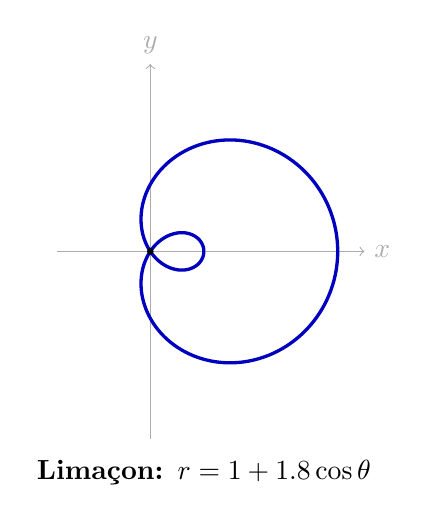
\begin{tikzpicture}[scale=.85]
\draw[->,gray!65] (-1.4,0)--(3.2,0) node[right] {$x$};
\draw[->,gray!65] (0,-2.8)--(0,2.8) node[above] {$y$};
\draw[blue!75!black,very thick,samples=360,domain=0:360,smooth,variable=\t]
  plot ({(1+1.8*cos(\t))*cos(\t)},{(1+1.8*cos(\t))*sin(\t)});
\fill (0,0) circle (1.4pt);
\node[font=\bfseries] at (.8,-3.3) {Lima\c{c}on: $r=1+1.8\cos\theta$};
\end{tikzpicture}
\end{document}
